%
\hsection{\crowsFoot{O}{OM}{P}{OM}}%
\label{sec:rm:op}%
%
\begin{figure}%
\centering%
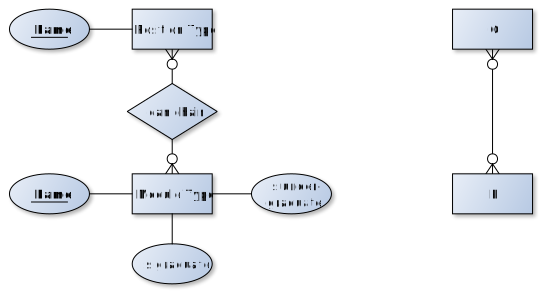
\includegraphics[width=0.86\linewidth]{\currentDir/OP}%
\caption{We encountered the \crowsFoot{O}{OM}{P}{OM} relationship pattern in \cref{fig:erdPersonStudentFaculty2}.}%
\label{fig:rm:op}%
\end{figure}%
%
\gitSQLAndOutput{\databasesCodeRepo}{conceptualToRelational}{OP_tables.sql}{relationships}{}{}{postgres.sh}{OP_tables}{%
The realization of a \crowsFoot{O}{OM}{P}{OM} conceptual relationship.%
}%
\gitSQLAndOutput{\databasesCodeRepo}{conceptualToRelational}{OP_insert_and_select.sql}{relationships}{}{}{postgres.sh}{OP_insert_and_select}{%
Inserting into and selecting data from the realization of an \crowsFoot{O}{OM}{P}{OM} conceptual relationship given in \cref{lst:OP_tables}.%
}%
%
\gitExec{cdtrmTableO}{\databasesCodeRepo}{conceptualToRelational}{../_scripts_/db_table_to_latex_table.sh relationships o oid;x}%
\gitExec{cdtrmTableP}{\databasesCodeRepo}{conceptualToRelational}{../_scripts_/db_table_to_latex_table.sh relationships p pid;y}%
\gitExec{cdtrmTableROP}{\databasesCodeRepo}{conceptualToRelational}{../_scripts_/db_table_to_latex_table.sh relationships relate_o_and_p fkoid;fkpid}%
%
\begin{figure}%
\centering%
\floatSep%
\input{\gitFile{cdtrmTableO}}%
\floatSep%
\input{\gitFile{cdtrmTableP}}%
\floatSep%
\input{\gitFile{cdtrmTableROP}}%
\floatSep%
\caption{The contents of the the three tables in the implementation of the \crowsFoot{O}{OM}{P}{OM} conceptual relationship after executing \cref{lst:OP_insert_and_select}.}%
\label{fig:rm:op:tables}%
\end{figure}%
%
\gitSQLAndOutput{\databasesCodeRepo}{conceptualToRelational}{OP_insert_error.sql}{relationships}{}{}{postgres.sh}{OP_insert_error}{%
Trying to relate two entities twice, which is of course not permitted in \emph{any} relationship pattern.%
}%
%
We have the two entity types~O and~P.
Each entity of type~O may be connected to zero, one, or multiple entities of type~P.
Each entity of type~P may be connected to zero, one, or multiple entities of type~O.

We encountered this pattern back in \cref{fig:erdPersonStudentFaculty2} when we modeled the relationship between the different types of modules and the different types of teacher position.
For example, maybe a lecturer can propose and chair a module of type elective specialization course.
The mandatory core module may only be chaired by a full professor, who is also permitted to chair elective specialization course.
The Master's (thesis module) supervision may only be available to teachers that hold the position Master's supervisor.
This means that each position may give a faculty member the credentials to chair zero, one, or many different types of modules.
At the same time, a module type may be chaired by teachers belonging to zero, one, or many position types, as illustrated in \cref{fig:rm:op}.
Granted, the situation where a module type cannot be chaired by any position type would be very strange.
This maybe a shortcoming of our model back then{\dots}

When implementing this pattern, we need a table~\sqlil{o} for the entities of type~O.
The primary key of this table be~\sqlil{oid} and there also will be the example attribute~\sqlil{x}.
We also need a table~\sqlil{p} for the entities of type~P, which gets the primary key~\sqlil{pid} and the example attribute~\sqlil{y}.
Now, since each row in~\sqlil{o} can be related to multiple rows in table~\sqlil{p} and vice versa, no two-table solution is possible.
This time, there is no way around it:
We need three tables.
But this three-table approach will look pretty much like the one in \cref{sec:rm:ab} for the \crowsFoot{A}{O1}{B}{O1}, but with different~\sqlil{UNIQUE} constraints.

In \cref{lst:OP_tables}, we add the table \sqlil{relate_o_and_p} which has two columns,~\sqlil{fkoid} and~\sqlil{fkpid}, which are foreign keys pointing to the primary keys~\sqlil{oid} and~\sqlil{pid} of tables~\sqlil{o} and~\sqlil{p}, respectively.
This is ensured with corresponding \sqlil{REFERENCES} constraints.
Both columns are marked as~\sqlil{NOT NULL}.
Neither of them is~\sqlil{UNIQUE}, because each row of table~\sqlil{o} can be related to multiple rows of table~\sqlil{p} and vice versa.
Still, the a pair~\sqlil{(fkoid, fkpid)} can appear only once in the table, because two specific rows in tables~\sqlil{o} and~\sqlil{p} can, of course, be related only once to each other.
We could enforce this with a constraint~\sqlil{UNIQUE (fkoid, fkpid)}.
However, the right solution here is to go directly for~\sqlil{PRIMARY KEY (fkoid, fkpid)}.
Our table needs a primary key, and here, the only possible primary key are the pairs of~\sqlil{(fkoid, fkpid)}.
And primary keys must be unique by default, so this constraint also covers the uniqueness.

In \cref{lst:OP_insert_and_select}, we now insert data into the two tables.
Since both relationship ends are optional, we can first enter some data into the tables~\sqlil{o} and~\sqlil{p}.
Then we can add the relationships between the rows of these tables by inserting rows into table~\sqlil{relate_o_and_p}.
The contents of all three tables after inserting the data are displayed in \cref{fig:rm:op:tables}.
If we want to recombine data from the two tables, we can do this with two \sqlil{INNER JOIN}~expressions.

During the above example, we inserted the row~\sqlil{(1, 1)} into table~\sqlil{relate_o_and_p}.
This row establishes that the row with primary key~\sqlil{oid = 1} of table~\sqlil{o} is related to the row with primary key~\sqlil{pid = 1} in table~\sqlil{p}.
In \cref{lst:OP_insert_error}, we try inserting the row again into~\sqlil{relate_o_and_p}.
Of course, no two rows can be related twice.
(It would make, for example, no sense to assign the same address twice to the same person.)
Thanks to the \sqlil{PRIMARY KEY} constraint that we attached to table~\sqlil{relate_o_and_p}, this insertion fails.%
%
\FloatBarrier%
\endhsection%
%
